%% This is file `elsarticle-template-1-num.tex',
%%
%% Copyright 2009 Elsevier Ltd
%%
%% This file is part of the 'Elsarticle Bundle'.
%% ---------------------------------------------
%%
%% It may be distributed under the conditions of the LaTeX Project Public
%% License, either version 1.2 of this license or (at your option) any
%% later version.  The latest version of this license is in
%%    http://www.latex-project.org/lppl.txt
%% and version 1.2 or later is part of all distributions of LaTeX
%% version 1999/12/01 or later.
%%
%% The list of all files belonging to the 'Elsarticle Bundle' is
%% given in the file `manifest.txt'.
%%
%% Template article for Elsevier's document class `elsarticle'
%% with numbered style bibliographic references
%%
%% $Id: elsarticle-template-1-num.tex 149 2009-10-08 05:01:15Z rishi $
%% $URL: http://lenova.river-valley.com/svn/elsbst/trunk/elsarticle-template-1-num.tex $
%%
\documentclass[preprint,12pt]{elsarticle}

%% Use the option review to obtain double line spacing
%% \documentclass[preprint,review,12pt]{elsarticle}

%% Use the options 1p,twocolumn; 3p; 3p,twocolumn; 5p; or 5p,twocolumn
%% for a journal layout:
%% \documentclass[final,1p,times]{elsarticle}
%% \documentclass[final,1p,times,twocolumn]{elsarticle}
%% \documentclass[final,3p,times]{elsarticle}
%% \documentclass[final,3p,times,twocolumn]{elsarticle}
%% \documentclass[final,5p,times]{elsarticle}
%% \documentclass[final,5p,times,twocolumn]{elsarticle}

%% if you use PostScript figures in your article
%% use the graphics package for simple commands
%% \usepackage{graphics}
%% or use the graphicx package for more complicated commands
%% \usepackage{graphicx}
%% or use the epsfig package if you prefer to use the old commands
%% \usepackage{epsfig}

%% The amssymb package provides various useful mathematical symbols
\usepackage{amssymb}
%% The amsthm package provides extended theorem environments
%% \usepackage{amsthm}

%% The lineno packages adds line numbers. Start line numbering with
%% \begin{linenumbers}, end it with \end{linenumbers}. Or switch it on
%% for the whole article with \linenumbers after \end{frontmatter}.
%% \usepackage{lineno}

%% natbib.sty is loaded by default. However, natbib options can be
%% provided with \biboptions{...} command. Following options are
%% valid:

%%   round  -  round parentheses are used (default)
%%   square -  square brackets are used   [option]
%%   curly  -  curly braces are used      {option}
%%   angle  -  angle brackets are used    <option>
%%   semicolon  -  multiple citations separated by semi-colon
%%   colon  - same as semicolon, an earlier confusion
%%   comma  -  separated by comma
%%   numbers-  selects numerical citations
%%   super  -  numerical citations as superscripts
%%   sort   -  sorts multiple citations according to order in ref. list
%%   sort&compress   -  like sort, but also compresses numerical citations
%%   compress - compresses without sorting
%%
%% \biboptions{comma,round}

% \biboptions{}


\journal{Science of Computer Programming}

\begin{document}

\begin{frontmatter}

%% Title, authors and addresses

%% use the tnoteref command within \title for footnotes;
%% use the tnotetext command for the associated footnote;
%% use the fnref command within \author or \address for footnotes;
%% use the fntext command for the associated footnote;
%% use the corref command within \author for corresponding author footnotes;
%% use the cortext command for the associated footnote;
%% use the ead command for the email address,
%% and the form \ead[url] for the home page:
%%
%% \title{Title\tnoteref{label1}}
%% \tnotetext[label1]{}
%% \author{Name\corref{cor1}\fnref{label2}}
%% \ead{email address}
%% \ead[url]{home page}
%% \fntext[label2]{}
%% \cortext[cor1]{}
%% \address{Address\fnref{label3}}
%% \fntext[label3]{}

\title{LDTA Tool Challenge}

%% use optional labels to link authors explicitly to addresses:
%% \author[label1,label2]{<author name>}
%% \address[label1]{<address>}
%% \address[label2]{<address>}

\author[tue]{Mark van den Brand}

% Please add your names below, we can sort out the order later.

\author[umn]{Eric Van Wyk}
\author[umn]{Ted Kaminski}

\author[lu]{Niklas Fors}
\author[lu]{G{\"o}rel Hedin}

\address[tue]{Technical University of Eindhoven, Eindhoven, The Netherlands}
\address[umn]{University of Minnesota, Minneapolis, MN, United States}
\address[lu]{Lund University, Lund, Sweden}

\begin{abstract}

An abstract goes here...

\end{abstract}

\begin{keyword}
%% keywords here, in the form: keyword \sep keyword

%% MSC codes here, in the form: \MSC code \sep code
%% or \MSC[2008] code \sep code (2000 is the default)

\end{keyword}

\end{frontmatter}

%%
%% Start line numbering here if you want
%%
% \linenumbers

%% main text
\section{Introduction}
\label{sec:intro}

\begin{itemize}
\item How to read the paper?
\item Systems involved
\item Scanning and parsing
\item Name analysis and type checking
\item Source to source translation and code generation
\item Handling of artifacts
\end{itemize}

\section{Oberon0}
\label{sec:oberon}
Oberon, levels, challenges and examples


% 3--8 Systems
% Please add an input line below for your paper section.  We can sort
% out the order of these later.

\newpage
\newcommand{\code}[1]{\texttt{#1}}

\section{Silver, a meta-language for language extension}

\subsection{Introduction to Silver}

Silver is an extensible attribute grammar system that
supports many modern attribute grammar features.  These include
higher-order\cite{vogt89}, reference~\cite{hedin00informatica}, and a
simplified notion of collection attributes~\cite{boyland05}.
%
Silver introduced \emph{forwarding} into an attribute grammar
setting~\cite{vanwyk02}, a mechanism that is useful for specifying
composable language extensions.
%
It also has a module system and supports separate compilation.
%
Silver is distributed with and coupled to Copper, an integrated parser
and context-aware scanner generator~\cite{vanwyk07gpce}.  As a
language, Silver has specific syntax for specifying the concrete and
lexical syntax of the object language.
%
In addition, Silver's type system supports parametric polymorphism and
a limited form of type inference which allows one to write lazy
functional programs in Silver~\cite{kaminski11sle}.



We have found Silver to be a convenient and expressive way to implement
translators for a variety of languages.  The main purpose for
developing Silver and Copper is to investigate extensible languages in
which a \emph{host language} is composed with a set of
independently-developed \emph{language extensions}.  This composition
of specifications of these components is to be performed automatically
by Silver and Copper and can thus be done at the direction of a
non-expert programmer.

Silver is both a (meta) language for language specifications, as well
as a tool that translates AG specifications to Java and concrete
syntax specifications to the input language for Copper.  Copper
generates the scanner and parser as Java code as well.  The resulting
Java code is compiled and packaged into a JAR file.  Silver
(implemented as a Silver specification) and Copper are both
distributed in source form under the LGPL licences and as executable
Java Jar files, making installation simple.


\paragraph{The organization of the Oberon0 specification in Silver}

To demonstrate Silver's support for highly modular language design, the
Oberon0 specification is organized in many different Silver modules,
called grammars.
%
A grammar can contain lexical and concrete syntax specifications as
well as attribute grammar specifications for defining language
semantics, optimizations, and translations.  
%
A Silver grammar can be organized hierarchically in a directory
structure and grammar names match this structure.  
%
%A grammar is composed of the specifications in all Silver files
%(ending with a \code{.sv} extension) in a directory, and the scope of
%specifications in one file include all other files in that grammar.
%
Grammars can \code{import} and \code{export} specifications from other grammars to
create grammar specifications that are composed of multiple grammars. 
%
Thus a language designer has a high degree of flexibility in how he or
she organizes the language specifications.

\begin{figure}
\begin{verbatim}
core
  concreteSyntax, abstractSyntax, typeChecking
constructs
  controlFlow, dataStructures, procedures  
    concreteSyntax, abstractSyntax, typeChecking
tasks
  codegenC
    core, dataStructures, procedures
components
  L1, L2, L3, L4, L5, T1, T2, T3, T5
artifacts
  A1, A2a, A2b, A3, A4, A5
\end{verbatim}
\caption{The directory structure of the Oberon0 specifications.}
\label{silver:fig:structure}
\end{figure}

The directory/grammar hierarchy for the Silver specifications for
Oberon0 (contained in a directory named \code{Oberon0}) is shown in
Figure~\ref{silver:fig:structure}.  The specifications for the Oberon0
language constructs in the languages L1 to L5 and the specifications
for the language processing tasks T1 to T5 are organized across three
directories in the \code{Oberon0} directory: \code{core},
\code{constructs}, and \code{tasks}.
%
The \code{core} directory contains grammars with specifications for
the language L1 and tasks T1, T2, and T3.
%
In it, the L1 lexical and concrete syntax specifications and the T1 pretty
printing task specifications are in the grammar in
\code{concreteSyntax}, the abstract syntax and T2 name analysis task
is in the grammar \code{abstractSyntax}, and the type checking task
(T3) is specified in the \code{typeChecking} directory.
%
This illustrates one possible organization of the specifications.  Of
interest is that attributes implementing name analysis are written
on the grammar productions defining the abstract syntax, so-called
\emph{abstract productions}, while the type
checking attributes for these productions are defined in so-called
\emph{aspect productions} which allow one to define new attributes for
existing grammar productions.

The \code{constructs} directory defines the languages features that
are added to create language level L2 (\code{controlFlow}), L3
(\code{dataStrucutes}), and L4 (\code{procedures}) and these are 
organized in the same manner as the L1 specification in \code{core}.
%
This organization is inverted in the \code{tasks/codegenC} directory
in which the C code generation task specification is separate from all
language construct definitions and it is split so the specifications
for this task for language constructs for language L1, L3, and L4 are
in different grammars (\code{core}, \code{dataStructures},
\code{procedures}).

What is missing from \code{tasks/codegenC} are specifications for code
generation for the for-loop and case-statement L2 constructs.  As we
will see in Section~\ref{silver:sec:transformation}, the C code
translation of these features come for free from the use of
forwarding.  The for-loop indicates that it is semantically equivalent
to a while-loop (in the core language) and automatically gets its C
code translations from that construct.  Thus the T5 code generation task
and the L2 control flow constructs are independent of one another.

The grammars in \code{components} directory compose the relevant
grammars from \code{core}, \code{constructs}, and \code{tasks} to form
the specific languages (L1 through L5) and tasks (T1 to T5).  The
\code{artifacts} directory contains grammars for the specific
artifacts A1 to A5 which do little more than import the appropriate
grammars from the components directory.  
%
Grammar composition is essentially the set union of the different
types of specifications in the various modules.
%
These grammars and the composition process are discussed in more
detail in Section~\ref{silver:sec:artifacts}


\subsection{Scanning and parsing}

Silver is coupled to our integrated parser and context-aware scanner
generator, Copper, and allows concrete and lexical syntax
specifications to be written in the same grammar modules as the
attribute grammar specifications.  These specifications are collected
and passed to Copper for analysis and generation of a context-aware
scanner and slightly modified LALR(1) parser that is used in the
resulting AG evaluator generated by Silver.

Copper has two distinguishing characteristics.  First, Copper generates
context-aware scanners~\cite{vanwyk07gpce} which use contextual
information to dis-ambiguate lexical syntax.
%
The parser uses a slightly modified LR- style algorithm that passes to
the scanner the set of valid symbols that the scanner may return at
that point in parsing. This set consists of the terminals whose
entries in the parse table for the current parse state are
\emph{shift}, \emph{reduce}, or \emph{accept}, but not \emph{error}.
The scanner will only return tokens in this set and a static analysis
ensures there are no lexical ambiguities; thus at most one token will
ever be returned from the scanner.

This type of scanning allows terminals that appear in different
parsing contexts to have overlapping regular expressions.  This is
especially useful when parsing and scanning extensible languages in
which domain specific languages can be embedded since the host and
embedded languages may have overlapping lexical syntax.  More
generally, this means that terminal symbols do not need to be
overloaded, instead different terminal symbols can be specified with
overlapping regular expressions.  This means that they are not
overloaded in the parser and thus parse table conflicts are less
likely to occur~\cite{vanwyk07gpce}.

Second, Copper comes with a modular determinism
analysis~\cite{schwerdfeger09pldi} that lets extension writers check
the concrete and lexical syntax specification of their extension to
ensure that the composition of the host language and any other
extensions verified by this analysis will be free of conflicts and
lexical ambiguities.  That is, the parser and scanner generated from
the composition ``just works.''

%  These are explained in more detail below when describing specific
%  Oberon0 specifications.

\paragraph{Sample specifications - lexical syntax}
While the scanning and parsing techniques used by Copper are different
from others, the structure of the specifications are quite familiar.
%
Specifications for lexical syntax consist primarily of terminal symbol
declarations, which, as expected, name the terminal symbol and provide
the defining regular expression.  In the Silver specification, the
\code{Id\_t} terminal specifies variable names:

\noindent
\verb!terminal Id_t /[A-Za-z][A-Za-z0-9]*/ ;!

Terminals such as keywords, punctuation, and operators, whose regular
expressions match only one string can specify the regular expression
as a string in single quotes as is done below for the assignment and
addition operator terminal symbols:

\noindent
\verb!terminal Assign_t ':='  ;! \\
\verb!terminal Plus_t   '+'  precedence = 11, association = left;! \\
%
Such terminals can be used in concrete productions by writing the
string in single quotes instead of using the terminal, which is
sometimes more convenient and can improve the readability of the
productions. 
%
This example also shows the use of traditional precedence and
associativity specifications.

Copper supports a notion of lexical precedence, for disambiguating
keywords from variables, for example, and the specification of
white-space and comments with a \code{ignore} modifier that indicates
a terminal is not to be passed on to the parser.


\paragraph{Sample specifications - concrete syntax}
Specifications for concrete syntax also have a familiar structure.
Figure~\ref{silver:fig:concrete} shows the specification of the two
for-loop constructs added in language L2.
\begin{figure}
\begin{verbatim}
concrete productions s::Stmt_c
 | 'FOR' id::Name_c ':=' lower::Expr_c 'TO' upper::Expr_c
                    'DO' body::Stmts_c 'END'         
  { s.ast = forStmt(id.ast, lower.ast, upper.ast, body.ast); }
 | 'FOR' id::Name_c ':=' lower::Expr_c 'TO' upper::Expr_c
                    'BY' step::Expr_c 'DO' body::Stmts_c 'END' 
  { s.ast = forStmtBy(id.ast, lower.ast, upper.ast, step.ast, 
                      body.ast); }
\end{verbatim}
\caption{Concrete syntax specifications for the for-loop.}
\label{silver:fig:concrete}
\end{figure}
These productions are written in the more-or-less familiar BNF-style.
Nonterminals and terminal symbols can be named and used in the
attribute definitions that can decorate concrete productions.  Here the
higher-order synthesized \code{ast} attribute is used to construct
ASTs.  Attribute definitions are specified between the curly braces
following the production definition.
%
For the first production, the abstract for-loop AST is stored
in the \code{ast} attribute of the left hand side nonterminal named
\code{s}. Since punctuation, for example \code{:=}, and keywords do
not appear in the AST, they are specified here using only the constant
lexeme in single quotes that was given in the definition of that
terminal symbol.

As we will see below, productions defining the abstract syntax of the
language differ from concrete production in only three ways: they use
the \code{abstract} modifier instead of \code{concrete}, they are named
unlike the anonymous productions shown in
Figure~\ref{silver:fig:concrete}, and they are not passed to Copper to
be used to generate a parser.  Otherwise there is no distinction
between the two in Silver.  Thus, one can define all the semantics of
the language on the concrete syntax tree if desired.  For Oberon0 we
chose to use a separate abstract syntax, primarily for demonstration
purposes.



\subsection{Name analysis}

Name analysis in the Silver implementation of Oberon0 proceeds in a standard
way: an environment exists to look up symbols, it's extended by declarations,
and consulted to report redeclarations or undefined symbols.
%
The environment is represented by the \texttt{env} inherited
 \footnote{Actually it is an 'autocopy' attribute, this is simply an inherited attribute
 that implicitly copies from parent to child if no other definition is present.}
attribute.
%
% TODO: should we be making references to where these are in the code?
%
The \texttt{Env} type is simply a container for the separate namespaces of the
environment.
%
Each names space (e.g. the \texttt{values} attribute on \texttt{Env}) has the
type \texttt{[TreeMap<String  Decorated Decl>]}.
%
The list represents \textit{scopes}, while the map allows looking up bound
names.

This representation is actually ``over powered" for Oberon0's needs.
%
Ober-on0 does not have separate namespaces for values and types, so our
separation of them in the environment is actually unnecessary, and in fact
adds a small complication to redeclaration checks: they must consult both
namespaces.
%
However, it is a nice demonstration of how a more interesting environment
would be set up.

%\paragraph{Extensible Records.}
%
% TODO: discuss whether we should have this section on how the environment is
% set up in a way that allows new namespaces to be added by extensions, making
% it, in effect, an extensible environment.

\paragraph{Decorated types}
The result type of looking up a name in the environment -- \texttt{Decorated Decl} --
is a \textit{reference attribute} to the node in the tree that declared that name.
%
Binding names to declaration sites is a relatively standard use for
reference attributes.
%
% TODO: we can cite JastAdd doing the same thing, probably, when we see their impl
%
Whereas a higher-order attribute only represents the \textit{structure} of
a tree, a reference attribute is actually a direct reference to an existing,
attributed, node in the tree.
%
Typically, reference attributes come along with some features for manipulating
them, such as \textit{remote attributes}.
%
Silver, however, treats them in a purely functional way; they can only be
consulted for the values of their attributes, and cannot be affected in
any way.
%
Reference attributes remain extremely useful, however, as this simplifies
many kinds of environment lookups.
%
For example, as we will see later, type checking and renaming transformations
can all proceed with no modifications to the environment: they simply consult
different attributes on the declaration node.

\paragraph{Specifications in a functional style}
The function \code{lookupType} is used to retrieve the reference to a
variable's declaration, if it exists, given the variables name and
environment.  The result \code{Maybe} type is constructed from either
a \code{nothing} or a \code{just} production.   This function is shown below:
\begin{verbatim}
function lookupType
Maybe<Decorated Decl> ::= s::String e::Decorated Env
{ return foldr(orElse, nothing(), lookupInScopes(s, e.types)); }
\end{verbatim}
It folds up the results of looking for the name \code{s} in all the
scopes in the the environment using a base-value of \code{nothing} and
combining results with \code{orElse} to return the first result from
\code{lookupInScopes} that is not a \code{nothing()}.
%
The function \code{lookupInScopes}, shown below,
\begin{verbatim}
function lookupInScopes
[Maybe<a>] ::= s::String ss::[TreeMap<String a>]
{ return map(adapt, map(treeLookup(s,_), ss)); }
\end{verbatim}
uses two applications of a
traditional polymorphic \code{map} function on the results of looking
up values in the underlying \code{TreeMap} structures.  (The
\code{adapt} function converts a list of values to a \code{nothing()}
if the list is empty or a \code{just} of the first element of the list.
Thanks to laziness, it's not inefficient to use this, as we'll only
actually do the lookup as far as gets demanded in the scope list.
This style of programming is quite familiar to functional programmers
and demonstrates the use of parametric polymorphism and higher-order
functions in Silver.


\paragraph{Collection attributes}
Silver's composition model allows extensions to \textit{safely} add new attributes
to existing nonterminals, as well as new productions, so long as those productions forward
to existing host language productions.
%
% This is very powerful.
%
It's worth noting that this is not easily possible
with objects nor algebraic datatypes, and is frequently called ``the expression
problem."
%
However, it's not a complete picture of composition.
%
Extensions may need to affect existing host language attributes in some ways.

The simplest example is error reporting: the host language defines a synthesized
attribute called \texttt{errors} that is simply a list of error messages.
%
However, extensions may need to add new error messages.
%
This is particularly apparent with our implementation, as type checking is
implemented separately from the core host language.

Silver provides a notion of \textit{collection attributes} that permits this.
%
Collection attributes are ordinary attributes that come with a
\textit{composition operator}, for example the \texttt{errors} attribute
is defined with the \texttt{++} (list append) operator:
%
\begin{verbatim}
synthesized attribute errors :: [Message] with ++;
\end{verbatim}
%
The term ``collection attribute" is somewhat overloaded, coming initially
from Boyland's remote attributes~\cite{boyland05}.
%
Silver's collection attributes do not permit any remote contribution across
the tree, however.
%
Instead, they are purely within one production, and contributions instead come
from all aspects of that production, along with an initial ``base" definition:
\begin{verbatim}
abstract production not
e::Expr ::= e1::Expr
{ e.errors := e1.errors;  -- Other attributes omitted
}
\end{verbatim}
%
% Thus, one could imagine a ``aspect weaving" phase of compiling a Silver
% program, where afterwards collections attributes have been ``erased" into
% normal attributes.
%
% The erased attribute equation would then look something like
% \texttt{foldr(compositionOperator, baseDef, [contribs...])},
% where the \texttt{contribs} list is has no specified order.
The final value of the collection attribute is equivalent to the
expression \texttt{foldr (} \emph{compositionOperator}\texttt{,}
    \emph{baseDefinition}\texttt{, [} \emph{contributions} \texttt{] )}.

This design is intended to tightly control the possible misbehavior of
extensions.
%
Extensions are forbidden from doing anything ``dangerous" by default,
and the host language can poke well-defined holes to permit specific
kinds of extension behavior.


\subsection{Type checking}

Typechecking is implemented separately from the host language, as some artifacts
lack it.
%
The typechecking extensions take the following form:
\begin{itemize}
\item A new attribute \texttt{type} occurs on \texttt{Decl}, and so can be
 consulted from the reference attribute returned by a name lookup in the
 environment.
\item That attribute is a new type called \texttt{TypeRep} that is a type
 representation, distinct from \texttt{TypeExpr} which represents program
 text of a type. Put another way, \texttt{TypeExpr} may need to look up things
 in the environment, and as a result yields a \texttt{TypeRep} which is totally
 self-contained.
\item Aspects for productions in the host language consult the environment
 and use the \texttt{errors} collection attribute to add error messages
 for type errors, for example with the previously mentioned \texttt{not} production:
\begin{verbatim}
  e.errors <- checkErrors(e1.type, booleanType(), 
                          "Operand to ~", e1.location);
\end{verbatim}
The function \code{checkErrors} returns a list containing a message if
the first two types do not match; the list is empty if they do.

\item Type equality checking is done using pattern matching, but also implemented
 in a way that allows it to be extended.
\end{itemize}

The distinction between type expressions and type representations is made for
convenience.
%
We could, instead, the same distinction already exists naturally:
\texttt{TypeExpr} and \texttt{Decorated TypeExpr} could serve the respective
roles.
%
However, much like the conversion from concrete to abstract syntax helps
avoid some unnecessary overhead in working with the abstract syntax, so
too does converting to \texttt{TypeRep}s.
%
In particular, new attributes added to type representations
(such as \texttt{mayPassByValue} added in the procedures extension) need not pay
any attention at all to name lookup in the environment.

The need for the distinction arises from where lookups of type names should
occur.
%
It is perfectly legal for a Oberon0 procedure to have a parameter of type
'Foo' that is an array of integers, and then to define the type 'Foo' in
its body to be a record.
%
The parameter type should still resolve as an integer.

To complicate things further, each of the types in the fields of a record should be
looked up and resolved where they occur in the program text, as well.
%
As a result, the \texttt{TypeRep} for records actually contains a reference
back to the \texttt{Decorated Decl} for the fields.


\paragraph{Pattern matching}
Although attributes are a powerful way of structuring most aspects of a compiler,
occasionally pattern matching becomes useful.
%
It is painful to write type equality checking code using just attributes,
similarly in any object-oriented language using just virtual methods
(where it would typically involve making restrictions on adding new types
and involve reflection or other hacks.)
%
Using pattern matching, however, can make it quite pleasant.

The type checking extension comes with a \texttt{check} function of two
\texttt{TypeRep}s that simply returns a boolean value.
%
In the host language, this simply matches integer/integer or boolean/boolean
to return true, otherwise it returns false.
%
However, this function is defined using another collection attribute,
this time using boolean-or as the composition operator.
%
In this way, each extension has an opportunity to examine the two types to
determine if that extension knows they are equal.
%
Should any extension say so, then \texttt{check} results in true.

To make error messages more manageable, there exists a special \texttt{TypeRep}
called \texttt{nominalTypeRep}, which does nothing but alter the ``pretty type"
of the type, and forward to the original \texttt{TypeRep} that it stands in for.
%
The advantage of this is that any error messages will now complain about the
actual types written in the code, rather than be expanded out to whatever
base representation a type has.
%
Silver gives a semantics to pattern matching~\cite{kaminski11sle} that makes it
behave more like what one would expect from working with attributes and
forwarding.
%
Specifically, the \texttt{check} function doesn't have to worry about this
production at all, because it will match as though it were the production
it forwarded to.

%\newpage
\subsection{Source-to-source transformation}
\label{silver:sec:transformation}


The Challenge task (T2) of adding a for-loop and case-statement to the
initial language, the code generation task (T5), and some simple
syntax desugaring all illustrate the effectiveness of
\emph{forwarding}, a mechanism for specifying attribute values that is
useful in writing composable language extensions.
%
In short, a production can compute, at attribute evaluation time, a
new syntax tree, called the ``forwards-to'' tree, from which it will
get default attribute values.  Any attribute not explicitly defined by
the ``forwarding'' production gets its value from the ``forwards-to''
tree.  It use in these tasks is described below.

\subsubsection{Desugaring}

The convenience provided by forwarding is apparent in the
specifications of the new T2 constructs: the for-loop and
case-statement.
%
On the
abstract productions for these constructs, we define
``front-end'' attributes such as those for reporting type errors on
the productions that define the new constructs so that error messages
are in terms of the constructs that the programmer wrote --- not those
the constructs may translate down to. 

The specification of the for-loop production \code{forStmtBy} is shown
below, with the expression defining \code{errors} and the computation to
generate the semantically-equivalent base language construct elided.
\begin{verbatim}
abstract production forStmtBy
s::Stmt ::= id::Name lower::Expr upper::Expr step::Expr body::Stmt
{ s.errors := ... ;
  forwards to ... assignment and while-loop implementing
                  the for-loop ... ;
}
\end{verbatim}
Since the ``back-end'' attributes for C code generation are left
undefined, the new production forwards to host language constructs
implementing the for-loop.  The code generated for this constructs is
simply the C code for their translations to an assignment and a
while-loop.  A similar process is used for the case-statement.


%\paragraph{Extensions, sugar, and dispatching}


%\paragraph{Syntaxtic sugar}
In addition to these T2 constructs, 
there are many language features that are often little more than easier or
more convenient ways of writing some other expression of identical meaning.
%
The host language we've defined for Oberon0 has one example: \texttt{VAR}
declarations can list multiple identifiers at once, with just one type.
%
That is, both \texttt{VAR x,y : INTEGER} and 
\texttt{VAR x : INTEGER, y : INTEGER} have the same meaning.
%
In the Silver implementation, the former declaration simply forwards to a sequence
of the latter kind of declarations.
%
This ``desugaring" acts similarly to a macro expansion, but with a critical
difference: the original tree is not lost or evaluated away.
%
Instead the original tree can still control the values of synthesized attributes.
%
For example, in order to prevent numerous error messages from being emitted,
it will only allow the \texttt{errors} attribute to forward through to the
expanded tree of declarations if there are no errors for the associated
type expression (i.e. the lookup succeeded.)
%
This is a common pattern with forwarding: still do error checking on the
``sugared" tree, so as to provide good error messages (unlike, say, template
errors in C++, or errors that occur within macro expansions in Lisp, or
the kind of error messages that result from complex type-level programming
in Haskell,) but otherwise let the ``expanded" tree do the real work (translation
and so forth.)

Forwarding is one of the major features of Silver that can dramatically
affect how specifications are written.
%
It ends up subsuming some of the role of many other features often found in
language processing tools: higher-order attributes, rewrite rules, desugaring,
inheritance, and macros. %, to start.

\subsubsection{Transformations for code generation}


The code-generation task (T5) is accomplished in Silver using
higher-order attributes to create the ``flattened'' Oberon0 program in
which all procedures are lifted to the top-level, as required by the
target language C.  We've implemented Johnnson's lambda-lifting
transformation~\cite{Johnsson85} to perform this task.
It requires first renaming variables so that all are unique and must
solve a set of recursive equations used to compute the
free-variables in recursive procedures that must now be passed in as
arguments.  Circular attributes would seem to be a natural fit for
solving these equations, but since Silver currently lacks these, the
equations are simply passed up to the top of the AST where they are
solved before the results are passed back down to where they can be
used.

\begin{comment}
\emph{To complete.}
\begin{itemize}

\item HOA used to create new, transformed, trees.

\item Two transformation merged into one pass in Oberon: renaming, and lambda lifting.

\item Renaming just threads a list of used names through the whole tree, and the
      resulting transformed tree just uses the reference attribute to find out the
      new name.

\item Lambda lifting moves all non-var declarations up to the
      top-level, in preparation for code generation.

\end{itemize}
\end{comment}

\subsubsection{Language Extensions}

%\paragraph{Language extensions}
The real advantage of forwarding is in specifying composable, yet
independently-developed language extensions.
%
While for desugaring, it is merely a convenience, for extension is it essential.
%
Without forwarding there is a problem resolving different kinds of extensions:
when one extension adds a new production, and another adds a new attribute,
what of the intersection of defining the value of this new attribute on the
new production?

For the Oberon0 specification, most of the components that are defined separately do
not qualify as ``composable" language extensions, because they do not have a
semantic equivalent in the host language.
%
For example, though it might be theoretically possible for procedures to
be translated away, it is not practical to do so.
%
In this case, the procedures extension must provide a conditional build trigger
to include its contributions to how translation to C should proceed, whenever both
these components are included.

But, for the control flow example, this is not necessary.
%
This is because the control flow extensions \textit{do} have semantic
equivalents in the host language.
%
The \texttt{FOR} and \texttt{CASE} statements forward to equivalent
\texttt{WHILE} and \texttt{IF} statements respectively.
%
As a result, any query for the values of attributes can simply be forwarded to
the equivalent tree in the host language where these attributes are defined.
%
It is worth pointing out that this functions despite some complexity in the
translation: it does renaming, and a full transformation of the tree, before
finally generating the C code.
%
And nowhere does any of it have to worry about these control flow statements.

\begin{comment}
% We say this above
The control flow extension \textit{does} provide equations for type checking,
however, for the same reason some type checking was done for desugaring previously:
error message quality.
%
Although the transformed trees should be semantically equivalent, that only
extends to whether it is accepted/rejected by analysis, not whether the error
messages generated are sensible.
%
It would be very confusing to see an error about an \texttt{IF} condition
not being a boolean when the program contains a \texttt{CASE} statement, instead.
%
By providing definitions for attributes involved in type checking, we can
get not only nice error messages, but also ensure the safety of composition.
\end{comment}

\begin{comment}
\paragraph{Dispatching} % We might cut this section for length TODO
Forwarding takes on many roles in Silver specifications.
%
One common one in larger compilers, that's we've forced to take a slightly
contrived role in Oberon0, is that of \textit{dispatch}.
%
It's often the case that the behavior of a production as a whole will end up
very different depending, for example, what kind of identifier is referenced
by a name, as determined by an environment lookup.
%
In the Silver compiler itself, for example, a global value lookup and a local
value do not just have very different translations, but the type behavior is
different too: globals are quantified and should have their type variable freshened
before reporting a monotype, while locals are not.

For Oberon0, we have a special handler for the builtin procedure \texttt{WriteLn}
and so forth, becuase we need to give them a special translation.
%
To do this, the procedure call production \texttt{callDispatch} forwards to one
of \texttt{call}, \texttt{writeLnCall}, etc based on the procedure name.
\end{comment}

\subsection{Code generation}

%\emph{To complete.}

This process is quite straight forward after the lambda-lifting
transformation has been made.  After that, all variable names are
unique and all procedures have been lifted up to the top level.  By
priming the renaming process with the C keywords, we can be assured
that they are not used as variable names.  Thus the generation of C
code boils down to little more than using a synthesized \code{String}
attribute to un-parse this Oberon0 AST using the concrete syntax of C.

\subsection{Artifacts (combination of tasks and sublanguages)}
\label{silver:sec:artifacts}

Stress the way that we can combine specs to create all the different
possibilities, not just the specified artifacts.

* grammar composition
* import statements
* parser specification
* build..with - a dependency on inclusion of other components.
  "It was used for problem X to include Y when Z was included."

\subsection{Observations}
\label{silver:sec:observations}

The Oberon0 specification highlights some of the strengths and
weaknesses of Silver.   The module system and use of forwarding allows
one to develop languages in a highly modular manner.   On the
other-hand, Silver is missing some helpful features such as a means for
specifying abstract trees using concrete syntax and a mechanism for
I/O that is less clumsy.

Like many language specification techniques, forwarding lets one build
up a language in layers, for example, the for-loop is built on top of
the core L1 language.  Forwarding allows us to avoid defining the
semantics (attributes) for some new constructs that can be seen as
syntactic sugar for those already existing in the language.  This is
seen in the fact that the for-loop gets it C translation from the L1
while-loop construct that it forwards/translates to.  But,
critically, it also allows to define attributes for some semantics,
for example type checking, when we want to do more than simply treat
the new constructs as macros that translate without any semantic
analysis down to other constructs.  In this case we provide
definitions for the type checking attributes so that better error
messages can be provided to the programmer.
%
Unlike many language specification techniques, forwarding does not
lock the language engineer into defining either all or none of the
semantics of a new language feature.

We were also pleased that we could specify the different artifacts of
the challenge in such a modular manner.  The composition model of
Silver is quite simple as it is just piece-wise set union of the
grammar specifications: grammars are set of productions, productions
(concrete, abstract, and aspect) have sets of attribute definitions,
and collection attributes are defined by sets of definitions spread
across different grammars.  This allows for the rather modular
specifications. 


On the other hand, there are some features and capabilities that
Silver is missing.   Below is a list of many of these.  (\emph{We're
  not sure all of these will be relevant for the paper, it depends a
  bit how we want the individual sections to say about these.   So our
  version of this may evolve after we've all had a chance to read
  drafts of each other's sections.})

\begin{itemize}
\item A mechanism for using the concrete syntax of code fragment in
  specifying what a production forwards to.  In the for-loop example
  we have to construct the AST that it forwards to using the abstract
  productions explicitly.   Something like the concrete syntax
  mechanisms in Stratego would be more convenient.   We've implemented a few
  prototypes to do this as composable language extensions to Silver,
  but they have a few rough edges.

\item Location information must be managed manually. This is tedious.
\item The ``back-door'' to the implementation Java language is really
  only useful to Silver developers.  In general we are not supporters
  of such back-doors, but they've been helpful in improving the space
  efficiency of Silver lists.  The bigger problem is that it is
  difficult to use Silver a component in language implementation in
  which parts are written Silver and other parts are written in Java
  or with some other language processing tool like those discussed in
  this paper.

\item Nested comments aren't yet possible.  This is a limitation of
  Copper since it works with regular expressions, not richer
  formalisms that would be needed to deal with nested comments.  

\item Silver can be seen as a pure lazy functional language, and thus
  safe I/O is a challenge.  An easy solution has been to adopt the use
  of an I/O ``token'' that is passed through side-effecting functions
  to schedule I/O in a predicable way.  This is a bit clumsy.

\item As a functional language is it missing a few important
  constructs such as function composition and lambda expressions.
  Type inference poses some challenges for attribute
  grammars~\cite{kaminski11sle} but a lambda expression that requires
  type annotations would not be too difficult to add.

\item Circular attributes would be helpful for tasks like lambda
  lifting and data flow analysis.
\item Silver currently lacks a static analysis to detect circularities
  in the attribute grammar.
\item There is no convenient way to do ``strategic'' or ``generic''
  programming so that once can, for example, specify that in the
  absence of an explicit definition for an attribute like
  \code{errors}, the value is computed by collecting and merging the
  lists of errors on the child nodes.
\item Silver currently has no IDE support, but this is something we
  are actively working to address.
\end{itemize}

\subsection{Conclusions}\label{silver:sec:conclusion}

To Do.

\lstnewenvironment{jastaddcode}
	{\lstset{
		basicstyle=\footnotesize\ttfamily,
		keywordstyle=\ttfamily\bfseries,
		commentstyle=\itshape\sffamily,
		tabsize=4,
		xleftmargin=0.2cm, %\parindent
		basewidth=0.6em,
		fontadjust= true,
		lineskip=0.7pt,
		aboveskip=\baselineskip,
		belowskip=\baselineskip,
		frame=tb,
		showspaces=false,
		showtabs=false,
		framerule=0.5pt,
		framexleftmargin=0.2cm,
		numbers=none,
		}
	}
	{}

\section{JastAdd}

%
% Introduction
%
\subsection{Introduction}
The JastAdd metacompilation tool~\cite{magnusson03scp} builds on object-oriented concepts: The abstract grammar is represented as a class hierarchy, and the abstract syntax tree (AST) as a tree of objects of those classes. The JastAdd specification formalism makes use of \emph{reference attributed grammars}~\cite{hedin00informatica} (RAGs), which extends Knuth's attribute grammars~\cite{knuth68mst}: An attribute is allowed to be a \emph{reference} to another node in the AST, and attributes in that node can be remotely accessed via the reference. For example, an Oberon-0 identifier has a reference attribute \texttt{decl} that points to the declaration of the identifier, and the identifier can find its type simply by remotely accessing the \texttt{type} attribute of its declaration, see Figure \ref{JA-UseDecl}.

A JastAdd specification declares a number of abstract grammar classes, attributes in such classes, and equations defining the values of those attributes. The specification is declarative in the sense that in an evaluated AST, the attributes will have values such that the equations hold. The order of evaluation is given implicitly, by the attribute dependencies in the equations, and evaluation is performed on demand \cite{jourdan84isp}. This declarative system can be integrated with imperative code that may read (but not write) attribute values. For example, the Oberon-0 code generator is implemented as methods that traverse the AST and output code to a file, reading attributes to decide what code to output. The AST is constructed by a parser, and attribute evaluation is then performed automatically, on demand, as attribute values are read.

A key feature of JastAdd is its modularity, allowing language constructs and computations to be modularized and extended. This is supported by the declarative computations (e.g., the order of equations is insignificant), the object-oriented foundation (e.g., classes can be extended through subclassing, and equations can be overridden in subclasses), and the use of inter-type declarations like in AspectJ \cite{kiczales01ecoop} (e.g., attributes of a class can be declared syntactically outside of the class).
For the Oberon-0 compiler, this is used to modularize the compiler according to the different artifacts, and the subproblems in those artifacts.

The JastAdd tool supports several kinds of attributes, and the ones used in the Oberon-0 compiler are summarized in Figure~\ref{JA-AttributeKinds}.

\begin{figure}
\begin{center}
\begin{tabular}{ | l c | l | l | }
  \hline             
  \multicolumn{2}{|l|}{\bf{attribute kind}} & \bf{description} & \bf{example use} \\
  \hline
  \hline          
  \emph{synthesized}& \multirow{2}{*}{\cite{knuth68mst}} & defined in the node & actual type \\
  \emph{inherited}& & defined in a parent node & expected type \\
  \hline 
  \emph{reference}& \multirow{2}{*}{\cite{hedin00informatica}}& can point to AST node & \multirow{2}{*}{name lookup}\\
  \emph{parameterized}& & can have argument & \\
  \hline
  \emph{non-terminal}& \cite{vogt89pldi}& a fresh AST subtree & predefined declaration \\
  \hline
  \emph{collection}& \cite{boyland98cc,magnusson09ase}& defined by set of partial values & compile-time errors \\
  \hline  
\end{tabular}
\caption{Attribute kinds used in the JastAdd Oberon-0 compiler.}
\label{JA-AttributeKinds}
\end{center}
\end{figure}


%
% Architecture and Parsing
%
\subsection{Architecture and Parsing}
A JastAdd specification consists a number of files with extensions \texttt{.ast} (abstract grammar), \texttt{.jrag} (attributes and their equations), and \texttt{.jadd} (imperative methods). The JastAdd tool is fed a number of these files as input, and produces Java source code as output. In this process, Java classes are generated corresponding to the abstract grammar in the \texttt{.ast} files, and code is woven into these classes, corresponding to the attributes, equations, and methods in the \texttt{.jrag} and \texttt{.jadd} files.

Scanning and parsing can be done with any tools that can create arbitrary Java objects as a result of the parse. For Oberon-0, the \emph{JFlex} scanner generator and the \emph{Beaver} parser generator are used, and code is added to the semantic actions of Beaver, to create ASTs according to the JastAdd abstract grammar.

To complete the compiler, a main program needs to be written in Java. The main program calls the parser to build the AST, and then produces some output based on the attributed AST, e.g., by calling a code generation method. Note that the main program does not need to invoke any evaluation code: as soon as the AST is built, its attributes can be accessed, since they are evaluated on demand. Figure~\ref{JA-GenerationProcess} shows a typical compiler generation process.

\begin{figure}[h]
\begin{center}
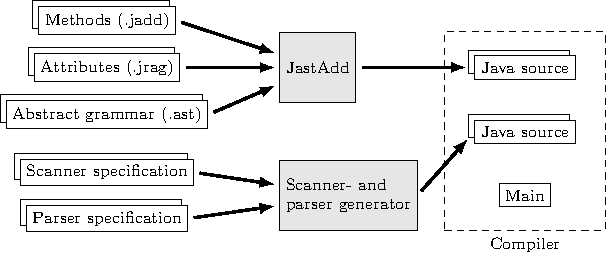
\includegraphics{jastadd/generation-process.pdf}
\caption{A typical compiler generation process using JastAdd.}
\label{JA-GenerationProcess}
\end{center}
\end{figure}

For the Oberon-0 compiler, the artifacts are specified in different directories: \texttt{A1}, \texttt{A2a}, \texttt{A2b}, \texttt{A3}, and \texttt{A4}. Within each directory, there are specification files for scanner, parser, abstract grammar, attributes, and methods. Typically, there are several attributes and methods files for different subproblems, e.g., name analysis, type checking, etc. Each artifact (except for \texttt{A1}) extends one or more previous artifacts, and its directory contains the specification files for that extension only. To build an artifact, an \emph{Ant} build file is used that simply lists all the relevant specification directories. This allows reuse of all the specification files from the previous artifacts, and only the build script and the main program need to be written specifically for the artifact. An explicit import mechanism would have been preferable to simply listing directories in the build script, but this is currently lacking in JastAdd. Figure~\ref{JA-ArtifactsOverview} shows all the specification files in the different artifact directories, their size, and how they depend on each other.

\begin{figure}[h]
\begin{center}
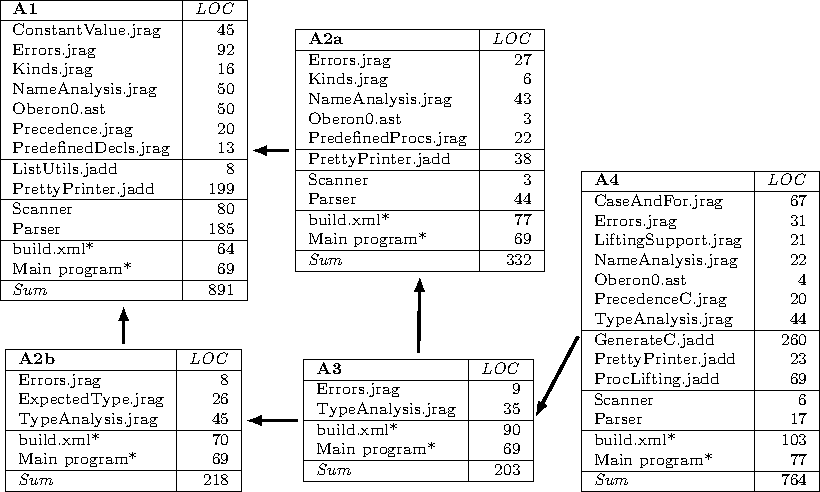
\includegraphics{jastadd/artifacts-overview.pdf}
\caption{An overview of modules in artifacts and how they extend each other. Arrow means extension and * means that the file is not reused.}
\label{JA-ArtifactsOverview}
\end{center}
\end{figure}

Figure~\ref{JA-AbsGram} shows some of the abstract grammar classes defined in the \texttt{A1} artifact. Abstract grammars are typically extended by adding new subclasses. For example, to extend Oberon-0 with procedures, a new class \texttt{Procedure} is defined in the \texttt{A2a} artifact, as a subclass of \texttt{Decl}.

\begin{figure}[h]\footnotesize
\begin{jastaddcode}
Module ::= <StartId> Decl* Block <EndId>; // The root class
abstract Decl;                     // Superclass for declarations
abstract Stmt;                     // Superclass for statements
Block : Stmt ::= Stmt*;            // Subclass for blocks
abstract Expr;                     // Superclass for expressions
abstract Access : Expr;            // Subclass for accesses
SimpleAccess : Access ::= IdUse;   // Subclass for access to simple var
IdDecl ::= <ID>;                   // Declared identifier
IdUse ::= <ID>;                    // Use of a declared identifier
...
\end{jastaddcode}
\vspace{-15pt}
\caption{Some of the abstract grammar classes defined in \texttt{A1/Oberon0.ast}. Tokens are enclosed in angle brackets. Lists are indicated by the Kleene star.}
\label{JA-AbsGram}
\end{figure}

Unfortunately, JFlex and Beaver do not support modularized specifications. For JFlex, we currently use a workaround by splitting the specification into several files, and concatenating them in different ways in the different build scripts. For Beaver, we use a preprocessor, called \emph{JastAddParser}, that has a specification similar to Beaver's, but where different productions can be specified in different files. This allows us to achieve the desired modularization also for the parsing, although in a somewhat clumsy way.


%
% Name analysis
%
\subsection{Name analysis}
\label{JA-NameAnalysis}
The task of name analysis is to bind an identifier usage to the corresponding declaration,
taking into account the language's scope rules. For Oberon-0, we represent identifier usages by the class \texttt{IdUse}, declarations by \texttt{IdDecl}, and bindings by a reference attribute \texttt{decl} in \texttt{IdUse}. The \texttt{decl }attribute is defined using an inherited parameterized attribute \texttt{lookup(String)}. This attribute is defined in some parent of the \texttt{IdUse}, typically in a procedure or a module, and will find the appropriate \texttt{IdDecl} node, given the identifier name as argument. This design makes it unnecessary to construct explicit symbol tables or environment data structures: we can instead use the AST itself as this structure. The Figure~\ref{JA-DeclNameAnalysis} shows part of the name analysis for artifact \texttt{A1}, and an example is shown in Figure~\ref{JA-UseDecl}. The equation in \texttt{Module} makes use of two other parameterized attributes, \texttt{localDeclLookup} and \texttt{localPredefinedLookup}, to delegate the search to the local declarations and the predefined declarations, respectively.

\begin{figure}
\begin{jastaddcode}
syn IdDecl IdUse.decl() = lookup(getID());
inh IdDecl IdUse.lookup(String name);
eq Module.getBlock().lookup(String name) {
    IdDecl decl = localDeclLookup(getNumDecl()-1, name);
    if (decl == null) decl = localPredefinedLookup(name);
    return decl;
}
\end{jastaddcode}
\vspace{-15pt}
\caption{Part of the name analysis for Oberon-0}
\label{JA-DeclNameAnalysis}
\end{figure}

\begin{figure}[h]
\begin{center}
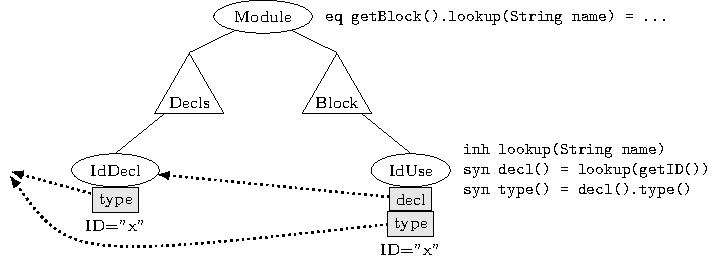
\includegraphics{jastadd/use-decl.pdf}
\caption{An AST illustrating how uses are bound to declarations, with the \texttt{decl} attribute. 
	Ellipses are AST nodes. Triangles are subtrees. Rectangles are attributes. 
	Solid lines are child/parent links. Dotted lines are reference values.}
\label{JA-UseDecl}
\end{center}
\end{figure}

In artifact \texttt{A2a}, procedures are added, and the name analysis needs to be extended with support for nested scopes. The Figure~\ref{JA-ProcNameAnalysis} shows how this is handled: The abstract syntax is extended with classes for \texttt{Procedure} and \texttt{ProcedureCallStmt}, and an equation for \texttt{lookup} is added in \texttt{Procedure}. The equation first searches locally among parameters and declarations in the procedure, and if no match is found there, the search is delegated to the context of the \texttt{Procedure}, using the l\texttt{ookup} attribute of the \texttt{Procedure} itself. This attribute is also declared in the figure, and will be defined by a parent \texttt{Module} or \texttt{Procedure} node, depending on the structure of the program.

\begin{figure}
\begin{jastaddcode}
Procedure : Decl ::= IdDecl ParDecl* Decl* Block <EndId>;
ProcedureCallStmt : Stmt ::= IdUse Expr*;

eq Procedure.getDecl(int index).lookup(String name) {
	IdDecl decl = localParLookup(name);
	if (decl == null) decl = localDeclLookup(index, name);
	if (decl == null) decl = lookup(name);
	return decl;
}
inh IdDecl Procedure.lookup(String name);
\end{jastaddcode}
\vspace{-15pt}
\caption{Extending Oberon-0 with procedures and nested name analysis} 
\label{JA-ProcNameAnalysis}
\end{figure}

In Oberon-0, constants, types, variables and procedures all use the same namespace. 
We can therefore use \texttt{IdDecl} and \texttt{IdUse} for all these
constructs, and share the definition of the \texttt{lookup} attribute between them.
To handle the \emph{declare before use} policy that applies within a declaration part, for example to look up type names, an additional parameter is used for \texttt{localDeclLookup}, to search only up to a certain point in the declaration list.

Oberon-0 contains a number of predefined declarations, e.g., the types \texttt{INTEGER} and \texttt{BOOLEAN}. In order to allow these to be handled in the same way as user-defined declarations, they are also represented in the AST. This is done using the NTA \texttt{predefinedDecls} in \texttt{Module}. A \emph{non-terminal attribute} (NTA) is both an attribute and an AST subtree at the same time, and is also called a \emph{higher-order attribute}~\cite{vogt89pldi}. The subtree of an NTA is created as the result of evaluating its defining equation. Figure~\ref{JA-PredefinedDecls} shows how a variable declaration uses the predefined type \texttt{INTEGER}, and how the \texttt{IdUse} of its type is bound to the \texttt{IdDecl} declaring \texttt{INTEGER} in the NTA.


%
% Type checking
%
\subsection{Type checking}
\label{JA-TypeChecking}

To typecheck an Oberon-0 expression, we compare its actual type with the type expected by its context. This is captured in two attributes: the inherited attribute \texttt{expectedType} and the synthesized attribute \texttt{type}. For example, for an assignment, the expected type of the right-hand side expression is the same as the type of the left-hand side variable, see Figure~\ref{JA-ExpectedType}.

\begin{figure}[h]
\begin{jastaddcode}
inh Type Expr.expectedType();

eq AssignmentStmt.getExpr().expectedType() = getAccess().type();
eq IfStmt.getExpr().expectedType() = module().boolType();
...
\end{jastaddcode}
\vspace{-15pt}
\caption{Definition of the inherited attribute \texttt{expectedType}}
\label{JA-ExpectedType}
\end{figure}

Type-checking errors, and other compile-time errors, are collected into a set-valued attribute \texttt{errors} in the \texttt{Module} node (the root of the AST). The \texttt{errors} attribute is a \emph{collection attribute}  \cite{boyland98cc,magnusson09ase} whose value is defined by \emph{contribution} rules, one for each possible compile-time error. 
Figure~\ref{JA-TypeErrors} shows how type-checking errors are collected, simply by contributing an error object when the actual and expected types are not compatible. Here, \texttt{error(String s)} is a method returning a fresh error object, \texttt{compatibleWith(Type~t)} is a parameterized synthesized attribute for comparing types, and \texttt{module()} is an inherited attribute returning the \texttt{Module} root node.

\begin{figure}[h]
\begin{jastaddcode}
Expr contributes error("Type error ...")
	when !type().compatibleWith(expectedType())
	to Module.errors() for module();
\end{jastaddcode}
\vspace{-15pt}
\caption{Collection of type checking errors}
\label{JA-TypeErrors}
\end{figure}

The synthesized attribute \texttt{type} is defined for the different kinds of expressions. For operators, the value is typically a predefined type, like \texttt{INTEGER} or \texttt{BOOLEAN}. The type of a variable or constant access is normally the type of its declaration. However, we also need to take into account that the declaration may be missing, or it may be a circularly defined constant, like \texttt{CONST c = c}. In these cases, we represent the type by an object \texttt{unknownType}, see Figure~\ref{JA-SimpleIdUse}. 

\begin{figure}
\begin{jastaddcode}
syn Type Expr.type();
eq RelationExpr.type() = module().boolType();
eq ArithmeticBinExpr.type() = module().integerType();
...
eq SimpleAccess.type() = getIdUse().type();

syn Type IdUse.type() {
	if (decl() == null || isCircular()) 
		return module().unknownType();
	return decl().type();
}
\end{jastaddcode}
\vspace{-15pt}
\caption{Definition of the synthesized attribute \texttt{type}}
\label{JA-SimpleIdUse}
\end{figure}

To resolve the type of a declaration, each \texttt{IdDecl} has an inherited attribute \texttt{type}. (Figure~\ref{JA-SimpleIdUse} showed an example use of the attribute.) Often, the type in a declaration is itself a use of a type declared elsewhere. It is then represented by a \texttt{TypeUse} node that contains an \texttt{IdUse} node which handles the name binding to the (type) declaration, just like for variables and constants. Figure~\ref{JA-PredefinedDecls} shows an example for the variable declaration \texttt{VAR~x~:~INTEGER;} The actual type of \texttt{x} is found by following the \texttt{decl} reference attribute in the type use. In this case, the type is located among the predefined declarations, in the NTA in the AST root.

\begin{figure}
\begin{center}
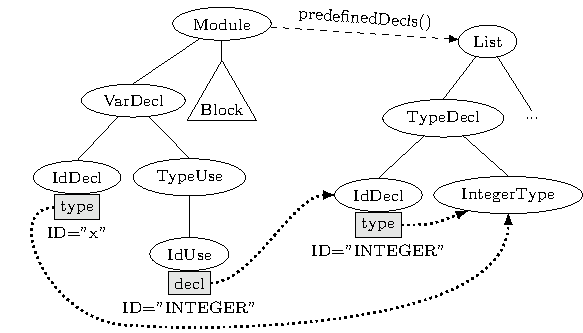
\includegraphics{jastadd/predefined-decls.pdf}
\caption{Shows binding of a type use, for \texttt{VAR x:INTEGER}, where \texttt{INTEGER} is a predefined type. Dashed lines are NTAs (e.g. \texttt{predefinedDecls}).}
\label{JA-PredefinedDecls}
\end{center}
\end{figure}


%
% Source-to-source transformation
%
\subsection{Source-to-source transformation}
Our implementation includes two kinds of source-to-source transformations: 1) procedure lifting in order to simplify generation of C code (since C functions cannot be nested), and 2) translating a larger language to a syntactically smaller core language, also to simplify code generation. 

Procedure lifting is implemented by generating a new AST where declarations of procedures, types and constants are moved to the top level. This is implemented as a method that traverses the original AST to build the new one, and uses attributes to decide what to build. For example, to generate new identifiers, the path from the root down to a declaration is used, and is captured by an inherited attribute \texttt{astPath} in \texttt{IdDecl}. The transformation is idempotent: applying the transformation more than once yields the same result. This is accomplished by using attributes to check if the original AST includes only top-level constructs.

To translate from a larger to a syntactically smaller language, NTAs are used. An example is translating \texttt{CASE} to \texttt{IF}.
This is done by defining an NTA \texttt{ifEquivalent} in \texttt{CaseStmt}. This simplifies code generation, since code can be generated for \texttt{CaseStmt} simply by delegating to the NTA. However, the NTA is only used for code generation: all compile-time error checking is still done directly in the original \texttt{CaseStmt}, in order to give error messages in terms of the original construct. The same technique is used to translate \texttt{FOR} to \texttt{WHILE}. Here, construction of the NTA is actually not simpler than just generating the code directly, but will pay off if several code generators for different targets are implemented.

%
% Code generation
%
\subsection{Code generation}
Generation of C code is implemented with a method \texttt{generateC}
that traverses the AST, making use of attributes to generate the correct code.
The code generation is similar to pretty printing, but needs to handle some additional things, like name collision with C's keywords, and that type declarations in C are structured in a somewhat different way. Parentheses are not stored in the AST, but are added during code generation and pretty printing, using attributes to encode the precedence rules.

To generate code for \texttt{CASE} and \texttt{FOR} is easy, it just amounts to delegating the work to the NTA. For example, the \texttt{ForStmt} class, delegates the code generation to its NTA \texttt{whileEquivalent}: 

\begin{jastaddcode}
public void ForStmt.generateC(StringBuilder sb, int indent) {
	whileEquivalent().generateC(sb, indent);
}
\end{jastaddcode}


%
%  Concluding observations
%
\subsection{Concluding observations}
\emph{Ease of use.} 
The main characteristic of JastAdd is its declarative specification technique that makes use of and blends with object-oriented programming: the AST is represented by an object-oriented model that arguably a normal OOP programmer would have constructed, but replaces imperative compiler phases with declarative computations in the form of attributes and equations.

In constructing the Oberon-0 compiler, we have reused a number of design ideas from earlier JastAdd compilers. These include:
\begin{itemize}
  \item Synthesized reference attributes, typically called \texttt{decl}, and inherited parameterized attributes, typically called \texttt{lookup}, for name analysis.
  \item Parameterized attributes that use double dispatch (calling another attribute) for comparing types~\cite{ekman07oopsla}.
  \item Collection attributes for collecting compile-time error messages.
  \item Non-terminal attributes for representing predefined declarations.
  \item Non-terminal attributes for representing new language constructs in terms of existing ones, in order to simplify code generation.
  \item Imperative methods that access attributes in order to implement pretty-printing and code generation.
\end{itemize}
We consider these design choices to be useful for most compiler implementations in JastAdd, and to demonstrate best practices in using the system.

\emph{Modularity.}
The declarative approach, together with the OO AST model and the use of AspectJ inter-type declarations, gives very strong support for modularization and extensibility. This is demonstrated by the Oberon-0 artifacts where all code except for the main programs and build files were reused in extensions. However, it should be noted that while extensions are often easy to add, it is not always completely straightforward. Sometimes, the base modules can be refactored to better support extension. We encountered one such example when arrays and records were to be added in artifact \texttt{A4}. Originally, artifact \texttt{A1} modeled variable accesses using a class \texttt{Access} that was a subclass to \texttt{Expr} and had an \texttt{IdUse} as its child:

\begin{jastaddcode}
Access : Expr ::= IdUse;
\end{jastaddcode}

However, when more complex accesses were added, like \texttt{ArrayElementAccess} and \texttt{RecordFieldAccess}, we needed them to subclass a more abstract \texttt{Access} class, since they had a different child structure. This was accomplished by refactoring \texttt{A1}, splitting the class \texttt{Access} into two: an abstract class \texttt{Access} and a subclass \texttt{SimpleAccess}, see Figure~\ref{JA-AbsGram}.

\emph{Analysis of specifications.}
JastAdd supports certain analysis of specifications: Static checks include checking that each attribute will have a defining equation for any possible AST. Dynamic checks include detection of cyclic evaluation (for attributes not declared as circular). We believe that the error messages are of reasonable quality. However, there is also room for improvement in several ways: The attribute equations are written in Java, and compile-time errors in them are not checked until compiling the generated Java code. While these errors are reasonably simple to map back to the equations in the JastAdd source code, it would have been better to get them directly in terms of that code. Furthermore, side effects are not allowed in the equations, but this is not checked, and may give rise to errors that are difficult to debug. This is something we would like to improve, for example by including an analysis similar to the the one proposed in the JPure system~\cite{pearce11cc}.

\emph{Performance.} JastAdd gives compilers of reasonable performance, as exemplified by the JastAdd Extensible Java compiler that performs within a factor of three in comparison to the Java reference compiler javac~\cite{ekman07oopsla}. 

To conclude, we think that the Oberon-0 implementation demonstrates well the language modularization capabilities of JastAdd, as well as many best practices for using the tool.


\section{Comparison of implementations}
\label{sec:comparison}
\begin{itemize}
\item Quantitative comparison (LoC)
\item Qualitative comparison
\end{itemize}

\section{Observations}
\label{sec:observations}

\section{Conclusions}
\label{sec:conclusions}



\appendix

\section{Oberon 0 code}
\label{sec:samples}
Appendix contains example of Oberon code with line numbers


%% The Appendices part is started with the command \appendix;
%% appendix sections are then done as normal sections
%% \appendix

%% \section{}
%% \label{}

%% References
%%
%% Following citation commands can be used in the body text:
%% Usage of \cite is as follows:
%%   \cite{key}          ==>>  [#]
%%   \cite[chap. 2]{key} ==>>  [#, chap. 2]
%%   \citet{key}         ==>>  Author [#]

%% References with bibTeX database:

%\bibliographystyle{model1-num-names}
\bibliographystyle{elsarticle-num}
\bibliography{silver/silver,jastadd/jastadd}

%% Authors are advised to submit their bibtex database files. They are
%% requested to list a bibtex style file in the manuscript if they do
%% not want to use model1-num-names.bst.

%% References without bibTeX database:

% \begin{thebibliography}{00}

%% \bibitem must have the following form:
%%   \bibitem{key}...
%%

% \bibitem{}

% \end{thebibliography}


\end{document}

%%
%% End of file `elsarticle-template-1-num.tex'.
